\section{Dormand-Prince (DOPRI54)}
\subsection{DOPRI54 with adaptive step size}
A special case of Runge-Kutta methods is the Dormand-Price. So relating to the general Runge-Kutta formulas in equation \ref{eq:RKgeneral1} and \ref{eq:RKgeneral2}, the Dormand-Prince method is obtained by choosing coefficients summarised by the following Butchers Tableau \cite{JrgensenRunge-KuttaEquations}:

\begin{table}[H]
\label{tab:DOPRI54}
\centering
%\caption{}
%\label{tab:q6_ButcherDOPRI54}
\begin{tabular}{c|ccccccc}
0 & 0 & 0 & 0 & 0 & 0 & 0 & 0 \\
$\frac{1}{3}$ & $\frac{1}{5}$ & 0 & 0 & 0 & 0 & 0 & 0 \\
$\frac{3}{10}$ & $\frac{3}{40}$ & $\frac{9}{40}$ & 0 & 0 & 0 & 0 & 0 \\
$\frac{4}{5}$ & $\frac{44}{45}$ & $\frac{-56}{15}$ & 0 & 0 & 0 & 0 & 0 \\
$\frac{8}{9}$ & $\frac{19372}{6561}$ & $\frac{-25360}{2187}$ & $\frac{64448}{6561}$ & $\frac{-212}{729}$ & 0 & 0 & 0 \\
1 & $\frac{9017}{3168}$ & $\frac{-355}{33}$ & $\frac{46732}{5247}$ & $\frac{49}{176}$ & $\frac{-5103}{18656}$ & 0 & 0 \\
1 & $\frac{35}{384}$ & 0 & $\frac{500}{1113}$ & $\frac{125}{192}$ & $\frac{-2187}{6784}$ & $\frac{11}{84}$ & 0 \\ \hline
 $x$ &  $\frac{35}{384}$ & 0 & $\frac{500}{1113}$ & $\frac{125}{192}$ & $\frac{-2187}{6784}$ & $\frac{11}{84}$ & 0  \\
$\hat{x}$ & $\frac{5179}{57600}$ & 0 & $\frac{7571}{16695}$ & $\frac{393}{640}$ & $\frac{-92079}{339200}$ & $\frac{187}{2100}$ & $\frac{1}{40}$ \\ \hline
$e$ & $\frac{71}{57600}$ & 0 & $\frac{-71}{16695}$ & $\frac{71}{1920}$ & $\frac{-17253}{339200}$ & $\frac{22}{525}$ & $\frac{-1}{40}$
\end{tabular}%
\caption{Butchers Tableau of DOPRI54.}
\end{table}

In other words, it has 7 stages and it is a 5th order method with a 4th order embedded method for error estimation. This means that the error the method commits from the exact solution is estimated by the difference between the 4th order solution from the more accurate 5th order solution: $e_n = x_n - \hat{x}_n = \Delta t_k \sum_{j=1}^{s} d_{j} f\left(T_{j}, X_{j}\right)$. The step size $\Delta t_n$ is then iteratively updated by

\begin{equation}
\Delta t_{n+1, j}=\left(\frac{\epsilon}{r_{n+1, j}}\right)^{\frac{1}{5+1}} \Delta t_{n, j}
\end{equation}

Over iterations of \textit{j}, until $r_{n+1, j} \leq 1$ where the step size is passed on $\Delta t_{n+1} = \Delta t_{n+1, j_{r\leq1}}$. $r_{n+1}$ is then calculated as
\begin{equation}
    r_{n+1} = \left\|e_{n+1}\right\|_\infty = \max _{p \in\{1, \ldots, P\}} \frac{\left|e_{p}\right|}{\mathrm{abs}_{p}+\left|x_{p}\right| \mathrm{rel}_{p}}
\end{equation}

Where \textit{P} is the dimension of $\boldsymbol{x}$. In this report, $\mathrm{abs}_p = \mathrm{rel}_p \quad \forall_p$ will be used.




%Often the power used is $\frac{1}{p+1}$ for when the embedded method is the one of highest order. However in this case the embedded method is of order 4 and therefore $\frac{1}{4+1}$ is used. \\
Since it is a 5th order method the local approximations error $l_n \propto (\Delta t_n)^{6}$.

\subsection{MATLAB implementation adaptive step size}
The following listing implements the DOPRI54 as described in the previous section.

\begin{adjustwidth*}{0cm}{-0.4cm}
\begin{lstlisting}[frame=single, language=Matlab,caption=DOPRI54, label=ERKpars]
function [Tout,Xout,Eout] = ...
        DOPRI54Adaptive(fun,tspan,x0,h,solver, ...
        abstol, reltol, varargin)

% Epsilon tolerance
epstol=0.8;

% DOPRI54 coefficients 
s = 7;
A = zeros(s,s);
A(2,1) = 1/5;
A(3,1) = 3/40;
A(4,1) = 44/45;
A(5,1) = 19372/6561;
A(6,1) = 9017/3168;
A(7,1) = 35/384;
A(3,2) = 9/40;
A(4,2) = -56/15;
A(5,2) = -25360/2187;
A(6,2) = -355/33;
A(4,3) = 32/9;
A(5,3) = 64448/6561;
A(6,3) = 46732/5247;
A(7,3) = 500/1113;
A(5,4) = -212/729;
A(6,4) = 49/176;
A(7,4) = 125/192;
A(6,5) = -5103/18656;
A(7,5) = -2187/6784;
A(7,6) = 11/84;
AT = A'
%bhat = [5179/57600; 0; 7571/16695; 393/640; -92097/339200; 187/2100; 1/40];
b = [35/384; 0; 500/1113; 125/192; -2187/6784; 11/84; 0];
c = [0; 1/5; 3/10; 4/5; 8/9; 1; 1];
d = [71/57600; 0; -71/16695; 71/1920; -17253/339200; 22/525; -1/40];
o = 5; % Order p=5
kpow  = 1/(o+1);     % kpow = 1/(order + 1)

h = h; % INIT

% Size parameters
x  = x0;                % Initial state
t  = tspan(1);          % Initial time
tf = tspan(end);        % Final time
nx = length(x0);        % System size (dim(x))

% Allocate memory
T  = zeros(1,s);        % Stage T
X  = zeros(nx,s);       % Stage X
F  = zeros(nx,s);       % Stage F

% More init
Tout = t;        
Xout = x';
Eout = 0;

% Algorithm starts here
while t < tf
    if (t+h > tf) % Don't go to far
        h = tf-t;
    end

    AcceptStep = false;
    while ~AcceptStep
        %%% Runge-Kutta
        % Stage 1
        T(1)   = t;
        X(:,1) = x;
        F(:,1) = fun(T(1),X(:,1),varargin{:});
        
        % Stage 2,3,...,s
        T(2:s) = t + h*c(2:s);
        for i=2:s
            X(:,i) = x + F(:,1:i-1)*h*AT(1:i-1,i);
            F(:,i) = feval(fun,T(i),X(:,i),varargin{:});
        end

        % Estimate of apprixmation error
        e = F*h*d;

        % Controlling step size h relative to error
        r = max(abs(e) ./ max(abstol, abs(x + F*h*b) .*reltol));
        h = (epstol/r)^(kpow) * h;

        AcceptStep = (r<=1.0);
        if AcceptStep
            t = t+h;
            x = x + F*h*b;
        end
    end
    % Save output when AcceptStep == true
    Tout = [Tout; t];
    Xout = [Xout; x'];
    Eout = [Eout; e];
end
\end{lstlisting}
\end{adjustwidth*}



\subsection{Test equation, order \& stability}
Considering again the test equation

$$
\dot{x}(t)=\lambda x(t), \quad x(0)=x_{0} \label{eq:test}
$$
With the analytical solution
$$
x(t) = \exp(\lambda t)
$$

And choosing $\lambda=-1$ and $x_{0}=1$ the approximated solutions as obtained by DOPRI54 is seen in Figure \ref{fig:6_3}. For a high tolerance the solution is quite off and with a decreasing tolerance the solution approaches that of the exact, analytical solution. Note how the DOPRI54 is not only far off the right solution, its embedded error estimation is also far off.\\

\begin{figure}[h]
    \centering
    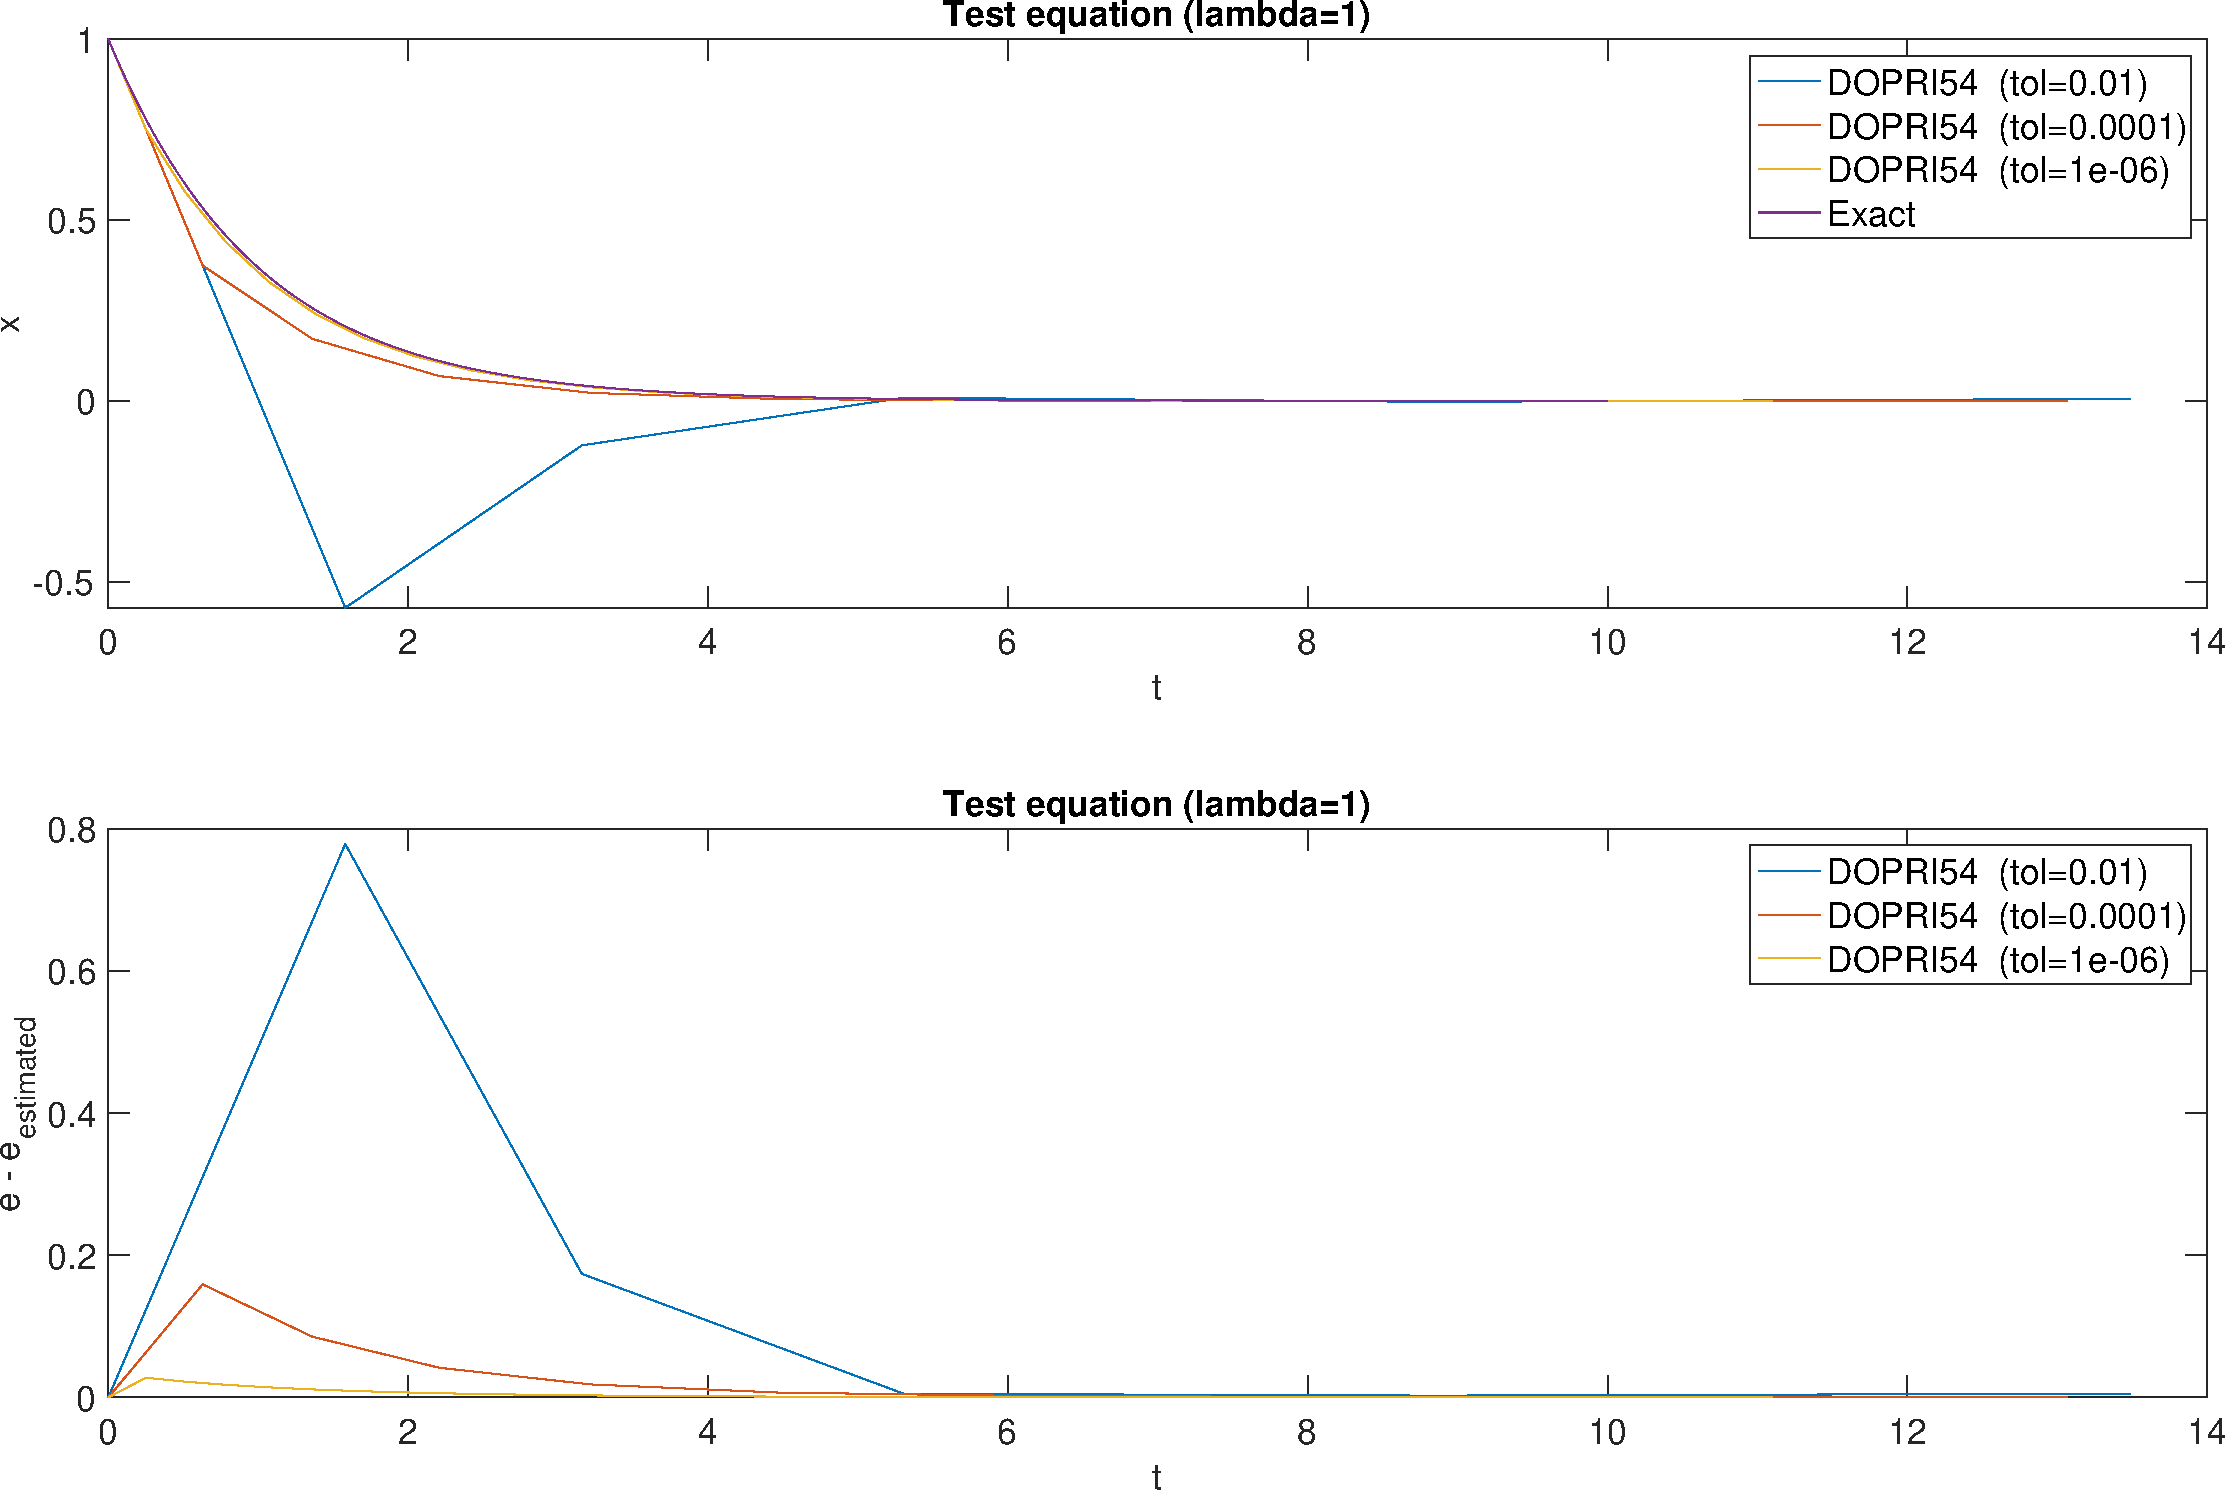
\includegraphics[width=\textwidth]{plots/6_3a.pdf}
    \caption{DOPRI54 solution on the test equation with $\lambda=-1$.}
    \label{fig:6_3}
\end{figure}

Now in terms of \textit{order} of the DOPRI54 method it has already been mentioned that it is a order 5 method. Let us verify that using the definition in Section 1.4. Recall that the order \textit{p} refers to the number of terms in the Taylor-expansion and that the local error is $l_{k}=\mathcal{O}\left(h_{k}^{p+1}\right)$. In Figure \ref{fig:6_3b} the local error of the DOPRI54 method is shown alongside other methods for context. Clearly it is method with higher accuracy. The slope of the linear line in the log-log plot is:

\begin{equation*}
    a_{DOPRI54} = 6.03 \implies p = 5 
\end{equation*}

I.e. DOPRI54 is a 5th order method.

\\\

Now in terms of \textit{stability}, the transfer function for any Runge-Kutta method is calculated as 

\begin{equation}
R(z)=1+z b^{\prime}(I-z A)^{-1} e
\end{equation}

Where $z = \lambda \cdot h$. By insertion of the relevant coefficients for the DOPRI54 as seen in Table \ref{tab:DOPRI54}, the resulting stability can be seen in Figure \ref{fig:6_3c}.

\begin{figure}[h]
    \centering
    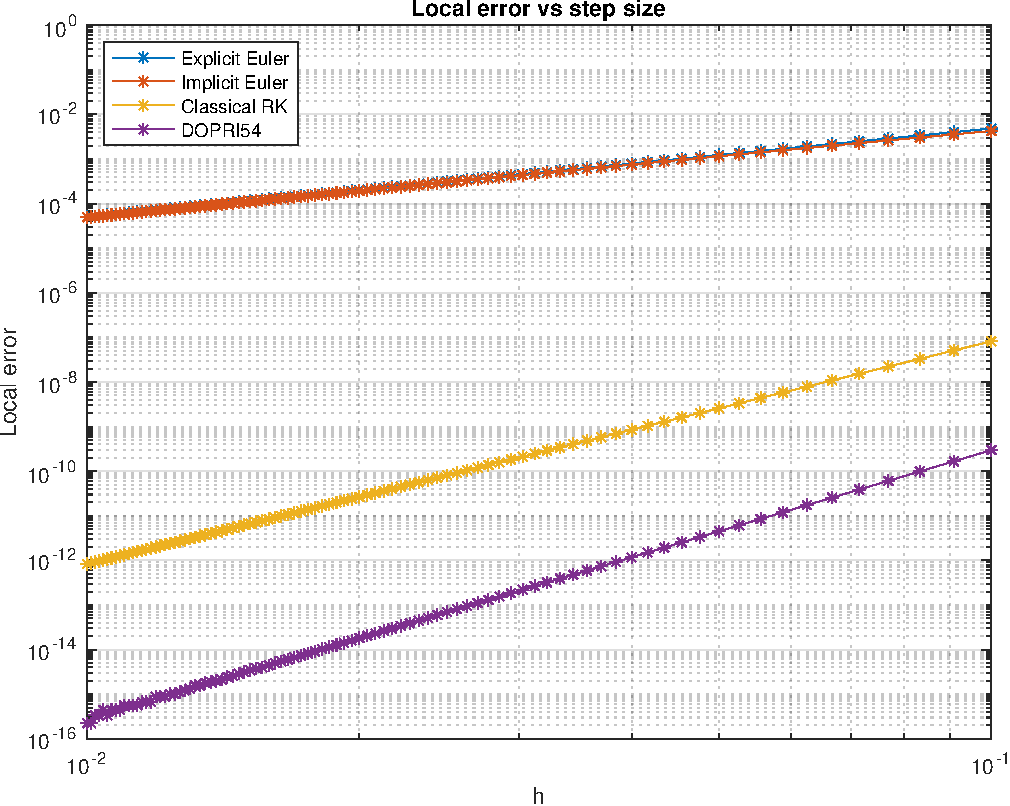
\includegraphics[width=0.7\textwidth]{plots/6_3b.pdf}
    \caption{Local error of DOPRI54 alongside other methods on the test equation.}
    \label{fig:6_3b}
\end{figure}

\begin{figure}[h]
    \centering
    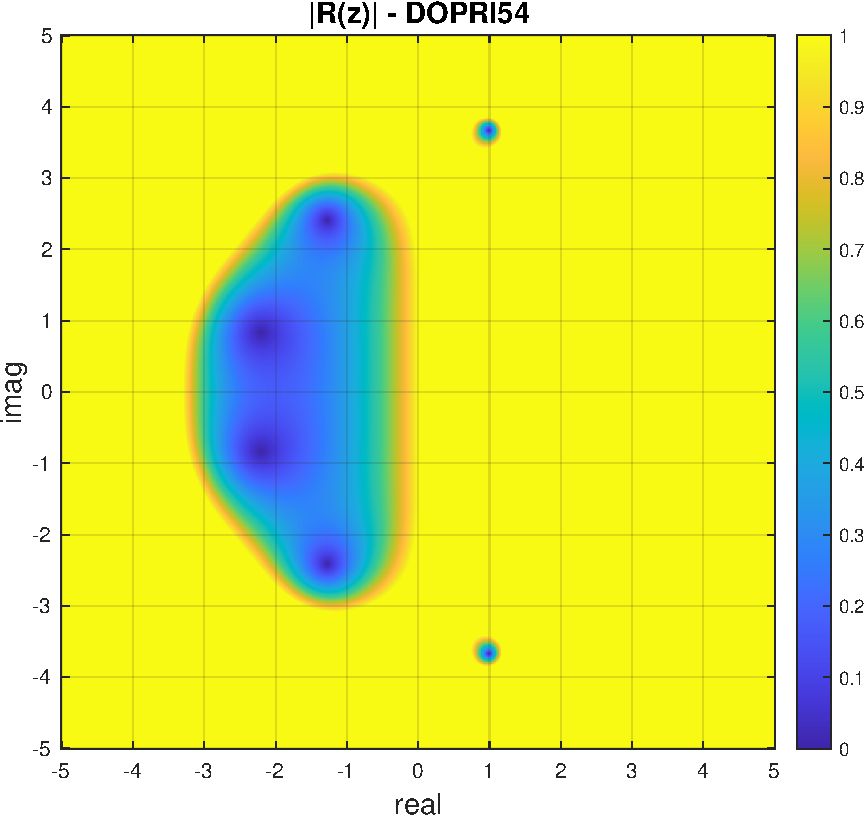
\includegraphics[width=0.7\textwidth]{plots/6_3c.pdf}
    \caption{Transfer function values for the DOPRI54 solution evaluated on $z = \lambda \cdot h$}
    \label{fig:6_3c}
\end{figure}

The non-yellow area is the stability regions of which $|R(z)| < 1$. Since $|R(z)| \geq 1$ for some $z$ where $Re(z) < 0$ the method is not A-stable and therefore neither L-stable.







\subsection{Van der Pol}
The results on applying the DOPRI54 implementation on the Van der Pol problem is seen in Figure \ref{fig:6_4}. Clearly the approximate solution becomes more and more accurate for lower tolerances. Additionally it is seen that it requires many more steps on the stiff problem. Interstingly, it requires fewer steps to ensure a $tol = 1e-04$ than $tol = 1e-02$ on the stiff problem. Since MATLAB'S \textit{ode45} is an implementation of the DOPRI54 a more thorough comparison between the two is presented in Section 6.6.

\begin{figure}[h]
    \centering
    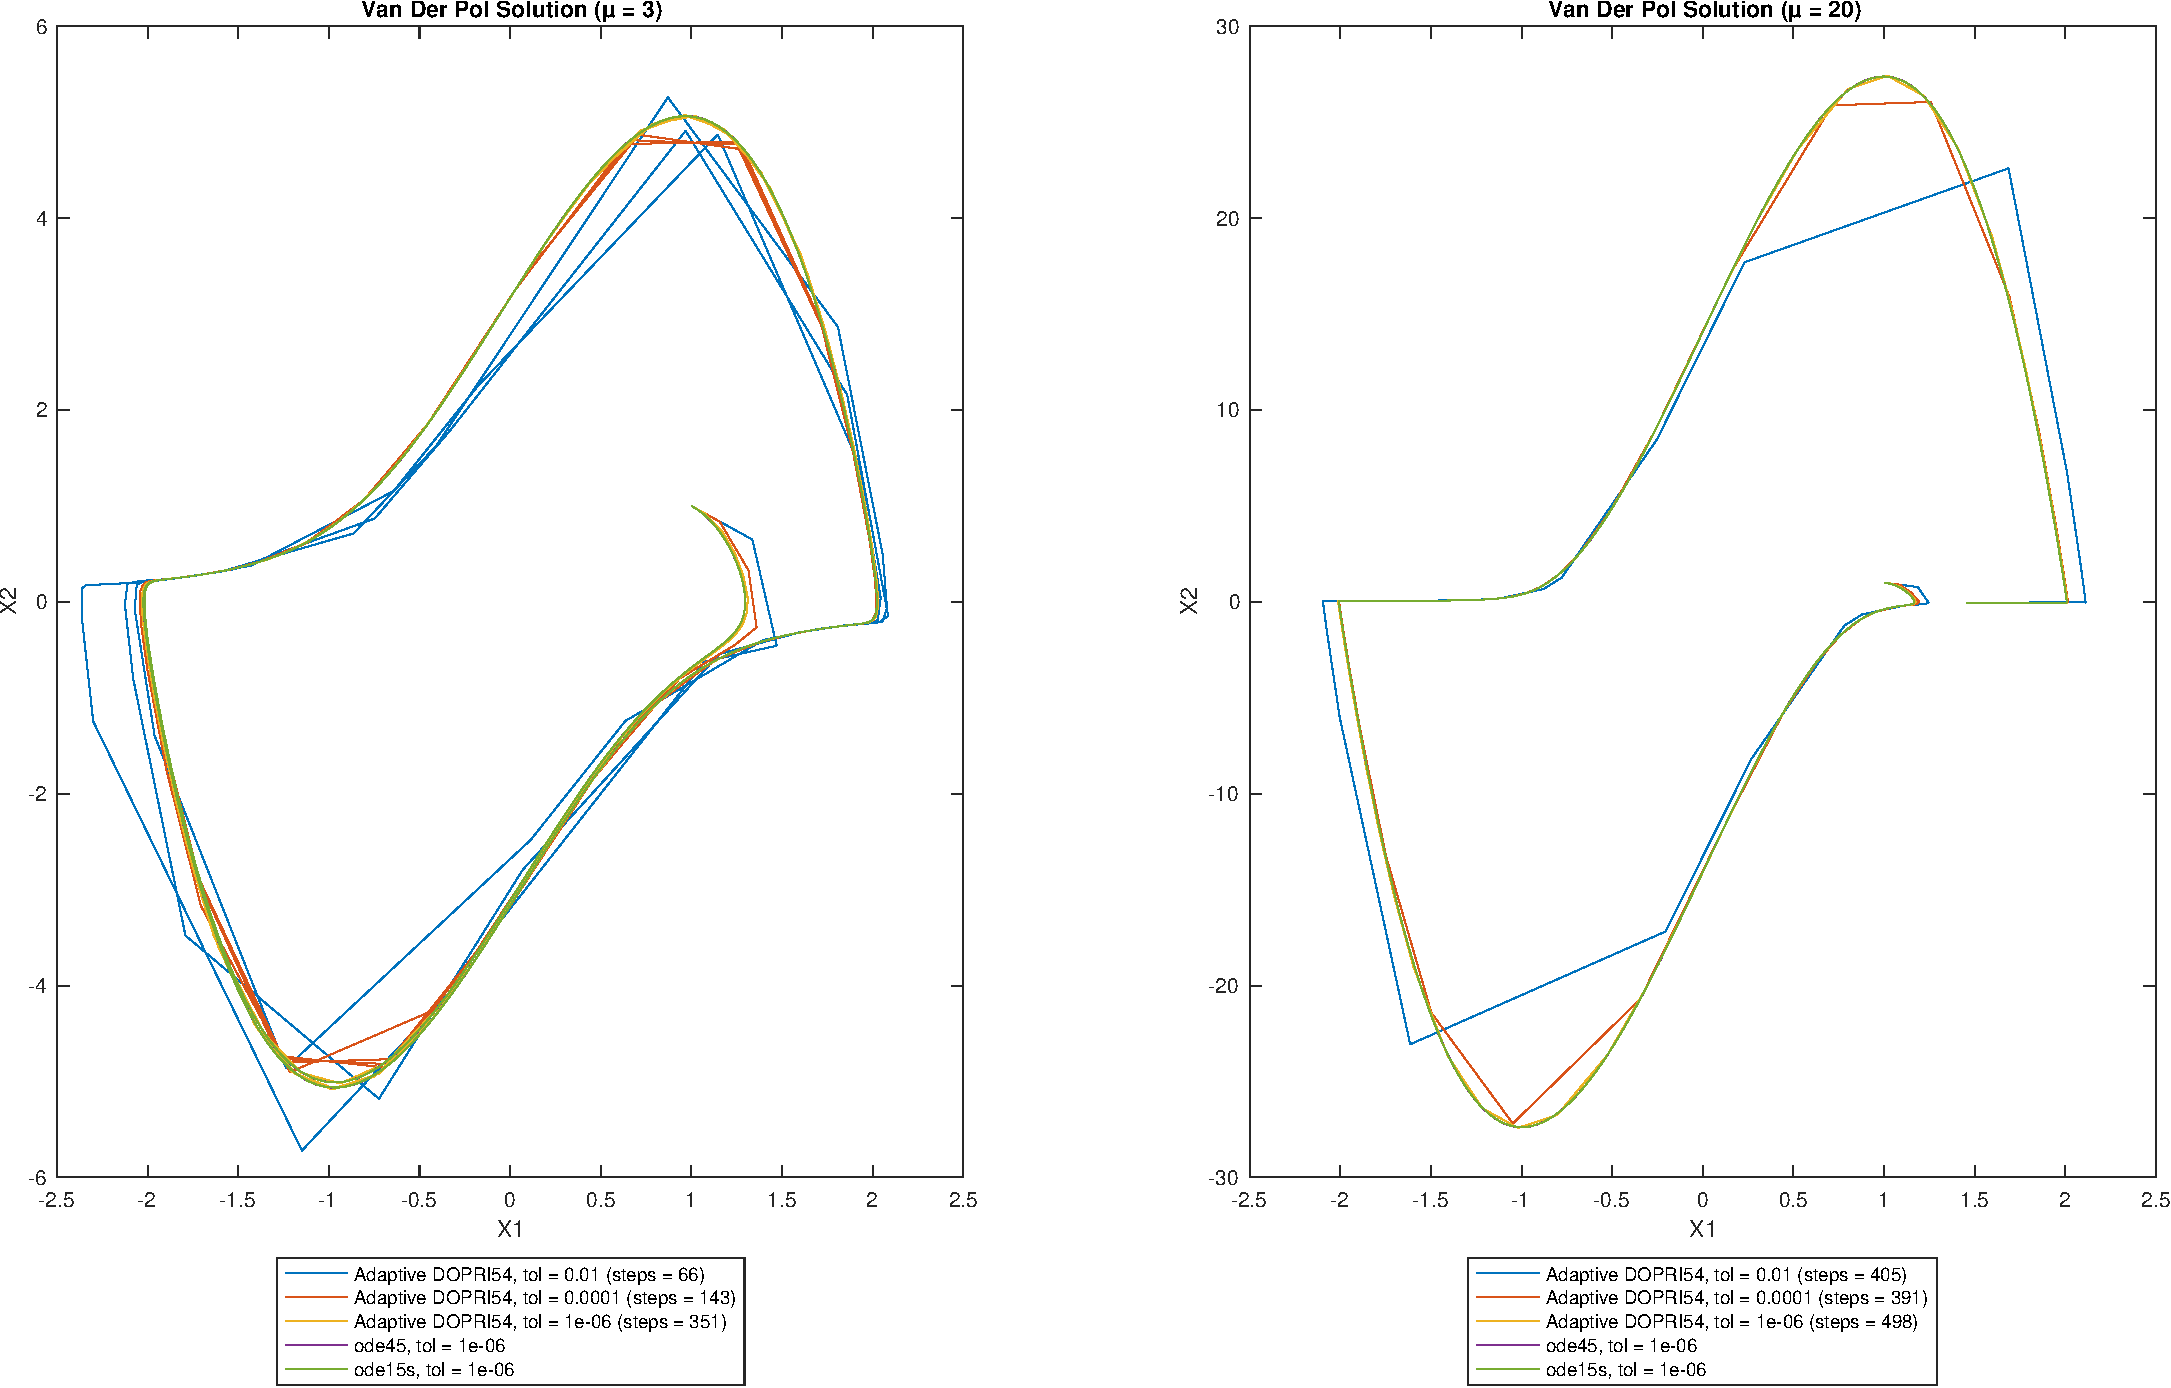
\includegraphics[width=\textwidth]{plots/6_5.pdf}
    \caption{Phase portrait of the Van der Pol solution using DOPRI54 as for a numerical approximation.}
    \label{fig:6_4}
\end{figure}






\subsection{Adiabatic Continuous Stirred Tank Reactor}
The Adiabatic Continuous Stirred Tank Reactor (CSTR) is a stoichiometric and exothermic model of the form (see \cite{Wahlgreen2020NonlinearCSTR} for details):

\begin{equation}
\begin{aligned}
\dot{C}_{A} &=\frac{F}{V}\left(C_{A, i n}-C_{A}\right)+R_{A}\left(C_{A}, C_{B}, T\right) \\
\dot{C}_{B} &=\frac{F}{V}\left(C_{B, i n}-C_{B}\right)+R_{B}\left(C_{A}, C_{B}, T\right) \\
\dot{T} &=\frac{F}{V}\left(T_{i n}-T\right)+R_{T}\left(C_{A}, C_{B}, T\right)
\end{aligned}
\end{equation}

i.e. a system of 3 ordinary differential equations. Where
\begin{equation}
\begin{aligned}
&R_{A}=R_{A}\left(C_{A}, C_{B}, T\right)=-r\left(C_{A}, C_{B}, T\right) \\
&R_{B}=R_{B}\left(C_{A}, C_{B}, T\right)=-2 r\left(C_{A}, C_{B}, T\right)\\
&R_{T}=R_{T}\left(C_{A}, C_{B}, T\right)=\beta r\left(C_{A}, C_{B}, T\right)
\end{aligned}
\end{equation}

Now in the following problem, the constants in Table \ref{tab:constants} are used.

\newcolumntype{L}{>{$}l<{$}} % math-mode version of "l" column type
\begin{table}[h]
\label{tab:constants}
\caption{Table summarising the constants used in the CSTR model}
\centering
\begin{tabular}{lLLL}
\hline
Density                  & \rho       & 1.0       & kg/L            \\
Heat capacity            & c_P        & 4.186     & kJ/(kg \cdot K) \\
Arrhenius constant       & k_0        & exp(24.6) & L/(mol \cdot s) \\
Activation energy        & E_a/R      & 8500      & K               \\
Reaction enthalpy        & \Delta H_r & -560      & kJ/mol          \\
Reactor volume           & V          & 0.105     & L               \\
Inlet concentration of A & C_{A,in}   & 1.6/2     & mol/L           \\
Inlet concentration of B & C_{B,in}   & 2.4/2     & mol/L           \\
Inlet temperature        & T_{in}     & 273.65    & K               \\  \hline
\end{tabular}
\end{table}

Now running the implemented DOPRI54 on this problem the solution can be seen in Figure \ref{}.

\subsubsection*{CSTR 1D}
Now the paper [ibid.] also suggests a 1-dimensional simplification of the 3-dimensional for when the exothermic dynamics is the main interest. The ODE is the formulated as

\begin{equation}
\dot{T}=\frac{F}{V}\left(T_{i n}-T\right)+R_{T}\left(C_{A}(T), C_{B}(T), T\right)
\end{equation}

The solution of running the DOPRI54 implementation on this problem can be seen in Figure \ref{}. Figure \ref{} compares the two implementations.


\subsection{Comparison with ode45}





























